\documentclass[11pt]{article}
\usepackage{bookmark}
\usepackage{algorithm}
\usepackage{algpseudocode}
\usepackage{amsfonts}
\usepackage{amsmath}
\usepackage{amssymb}
\usepackage{amsthm}
\usepackage{bm}
\usepackage{color}
\usepackage{comment}
\usepackage{float}
\usepackage{graphicx}
%\usepackage[hidelinks]{hyperref}
\usepackage{makecell}
\usepackage[caption=false,font=footnotesize,subrefformat=parens,labelformat=parens]{subfig}
\usepackage{wrapfig}
\usepackage{url}
\usepackage[table]{xcolor}
\graphicspath{{images/}}
\setlength{\parindent}{0.25in}
\setlength{\parskip}{.05in}
\pagestyle{plain}
%Title, date an author of the document
\title{Progress Report}
\author{Bardia Mojra}


\begin{document}
\maketitle
\thispagestyle{empty}

\bigskip
\bigskip
\begin{center}
 Robotic Vision Lab
\end{center}

\begin{center}
The University of Texas at Arlington
\end{center}

\newpage



\section{Progress}
The following items are listed in the order of priority:
\begin{itemize}
  \item DLO Dataset (\textcolor{red}{March 1st.}): This week, Maicol and I
  collected initial measurements for DLO dataset. We tested L515 LiDAR in different
  ambient light settings. L515 datasheet and user guide recommend operating the
  device in indoor environments and avoid sunlight as much as possible. We
  made various recordings of four DLOs in different light settings, i.e., at noon,
  at sunset, and after sunset. We did not observe a considerable difference between
  the measurements but we lack a systematic method for quantitatively measuring the
  effects of sunlight on DLO configuration estimation. See figures 1-4.\

  \begin{figure}[h]
    \caption{DLOs}
    \includegraphics[width=8cm]{side_01.png}
    \centering
  \end{figure}


  \begin{figure}[h]
    \caption{DLOs}
    \includegraphics[width=8cm]{side_02.png}
    \centering
  \end{figure}

  \begin{figure}[h]
    \caption{DLOs}
    \includegraphics[width=8cm]{side_03.png}
    \centering
  \end{figure}

  \begin{figure}[h]
    \caption{DLOs}
    \includegraphics[width=8cm]{top.png}
    \centering
  \end{figure}


  Perhaps, it would be useful in our paper if we
  provide information regarding ambient light (in lux) and how it effects our
  measurements and configuration estimation of DLO. The DLOs include a thick hose
  (part number and description needed), a AWG 10 red and black and CAT-6 bundle,
  a CSA LL90485 Water resistant with three AWG 16 conductors, a yellow Southwire
  E51583(UL) AWG 14 wire. See figure 5.\\


  \begin{figure}[h]
    \caption{DLOs}
    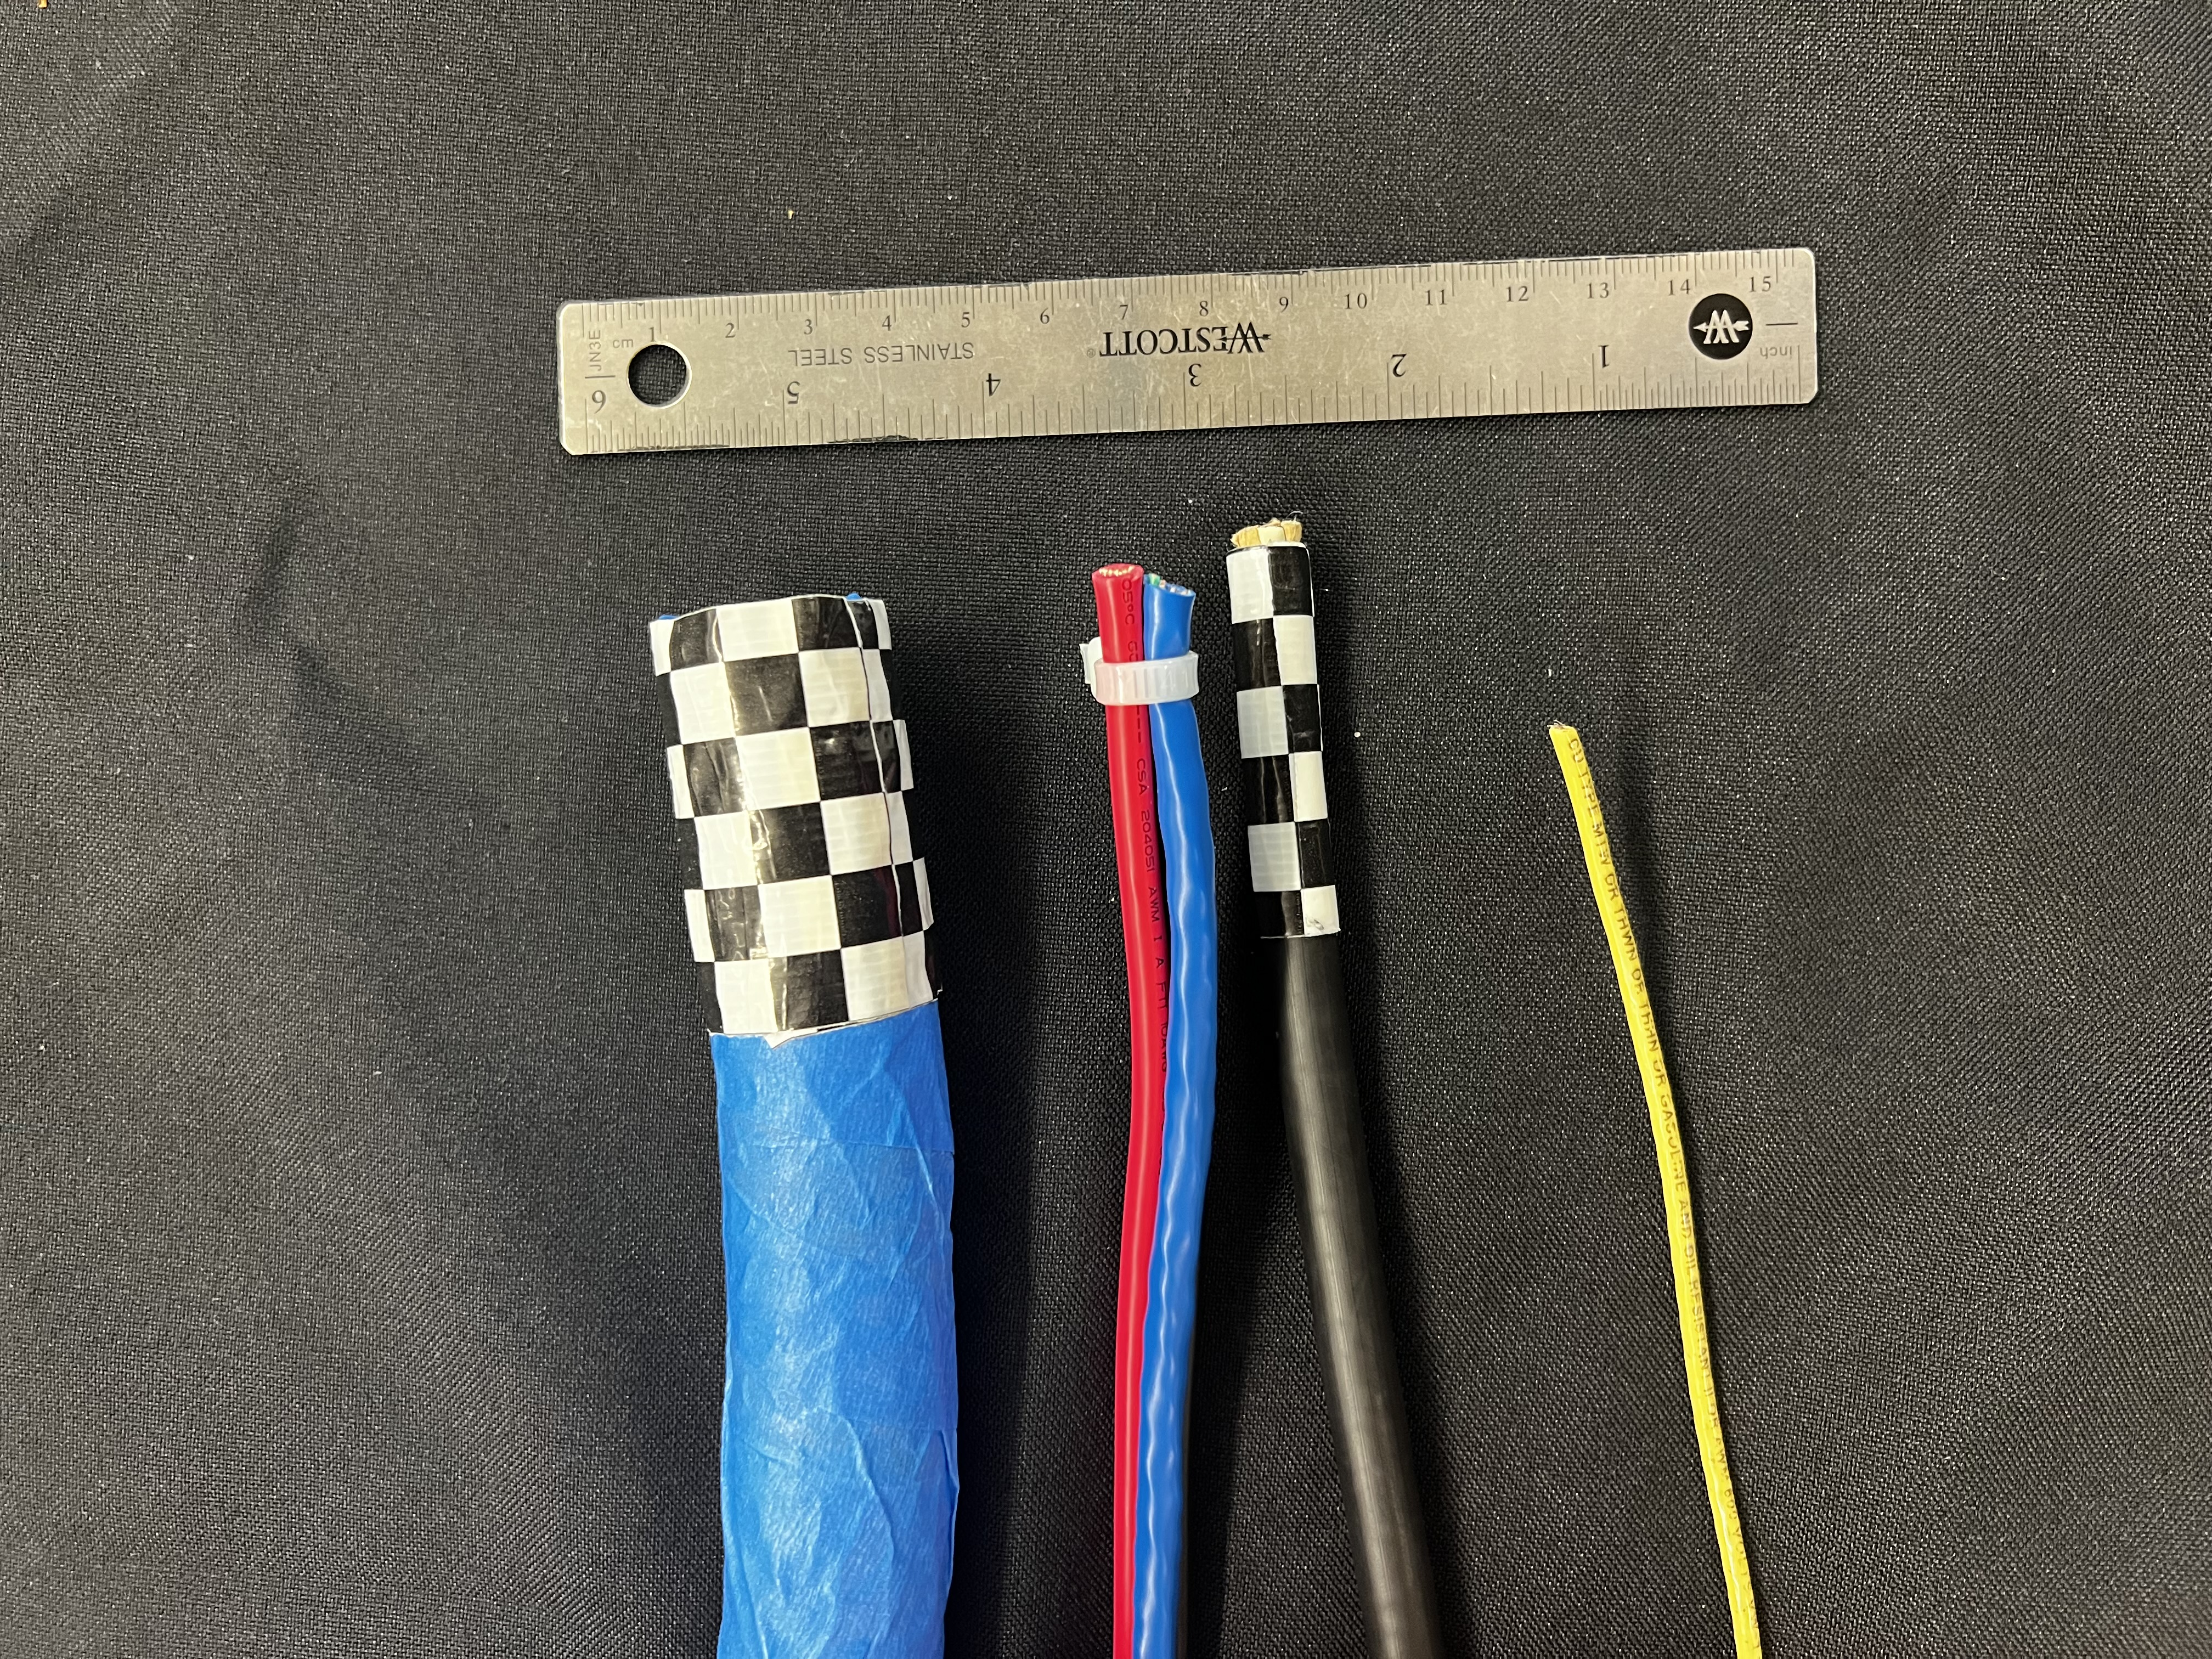
\includegraphics[width=8cm]{DLOs}
    \centering
  \end{figure}

  Currently, I am working on extracting the DLO shape from raw data.

  \item DLO Manipulation (\textcolor{red}{IROS}): \cite{abraham2017model}.\\
  \item Maicol (REU): //
  \item XEst (\textcolor{red}{RAL ---}): No update.\\
  \end{itemize}
\newpage

%Sets the bibliography style to UNSRT and import the
\newpage
\bibliography{ref}
\bibliographystyle{ieeetr}

\section{Research Plan - Out of date}
This section outlines my current research plan where the main ideas, target
conference/journal, and expected date of completion for each paper
are provided.
Target conferences: ICRA, IROS (March), CASE (Late Feb.), NIPS.
Target Journals: RAL, CVPR, CORAL.

\begin{itemize}
  \item Koopman-01 (\textcolor{red}{IROS - Dec. 1st - active}):
  Koopman-based MPC control of VTOL-DIP and VTOL-TIP in simulation,
  DLO pose estimation in simulation,
  experiments on choice of basis function and lifting dimensions,
  and performance comparison with optimal, robust, and/or
  adaptive control schemes.\
  \item Koopman-02 (\textcolor{red}{ACC - Sep 30th - active}):
  A review on Koopman-based control schemes. \textcolor{red}{Not enough, make
  it part of another paper.} Read papers and write literature reviews.\

  \item Koopman-03 (\textcolor{black}{RAL - Mar. 1st - status}):
  Extension to Koopman-01, Koopman-based dynamic estimation of DLO,
  collect dynamic DLO dataset,
  prediction of DLO configuration.

  \item Quest-01 (\textcolor{orange}{IROS - Mar. 1st - next}):
  Optimal transform solution for QuEst based on dominant mode decomposition (DMD).

\end{itemize}
\end{document}
